%=========================================================
\section{Actores del sistema}

Los actores son los perfiles asociados a las diversas áreas que intervienen en el proceso. Se han identificado los actores de acuerdo a las actividades y responsabilidades dentro del sistema, los cuales se muestran en la figura \ref{fig:perfiles} y se describen a continuación.

%    Los actores son los perfiles asociados a las diversas áreas y/u organizaciones que intervienen en el proceso. Se han identificado los actores de acuerdo a las actividades y responsabilidades dentro del \paear respecto al módulo de \textbf{Registro de escuelas}, los cuales se muestran en la figura \ref{fig:perfilesPAEAR} y se describen a continuación. 
    %y responsabilidades dentro del \paear - \saear, los cuales se describen a continuación.

    \begin{figure}[htbp!]
      \begin{center}
	  %\fbox{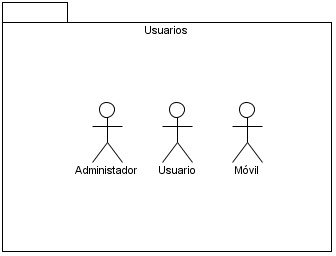
\includegraphics[width=0.7\textwidth]{ModeloComportamiento/imagenes/Actores.png}}
      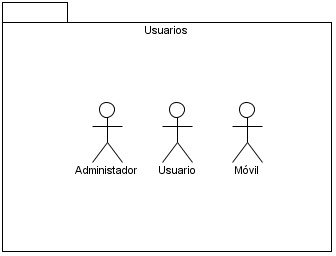
\includegraphics[width=0.6\textwidth]{ModeloComportamiento/imagenes/Actores.png}
      \caption{Perfiles identificados.}
      \label{fig:perfiles}
      \end{center}
    \end{figure}

%--------------------------------------------------------------------------------------------------
\begin{actor}{Paciente}{paciente}{Representa a cualquier persona de la que se requiere el monitoreo continuo de su frecuencia cardíaca y temperatura corporal.}

	\item[Cantidad:] Uno por sistema embebido.

\end{actor}
%
%\begin{actor}{Usuario}{usuario}{Representa a cualquier persona que requiera monitorear la frecuencia cardíaca y temperatura corporal de un paciente.}
%	
%	\item[Cantidad:] Uno por sistema embebido.
%	
%\end{actor}
%
%\begin{actor}{Sistema}{sistema}{Representa el sistema embebido compuesto por el microcontrolador, los sensores de pulso cardíaco y temperatura, y el módulo GSM.}
%	
%\end{actor}